\subsection{Mätningar} \label{sec:measurements}

Provernas (se avsnitt~\ref{sec:samples}) natur visas i
tabell~\ref{tab:samples}. Angiven ``strålning'' syftar på den typ av strålning
som undersökts för provet.

\begin{table}[!hp]
    \begin{tabular}{|l|l|l|l|l|l|}
    \hline
    Provets typ & Massa (\unit{g}) & Strålning & Pulser      & Mättid (\unit{s}) & Frekvens (\unit{\Hz}) \\
    \hline
    Svamp       & \num{18.0}       & $\gamma$  & \num{10977} & \num{804}         & \num{13.7}            \\
    \hline
    Salt        & \num{70.0}       & $\gamma$  & \num{314}   & \num{300}         & \num{1.05}            \\
    \hline
    Stav Cs-137 & -                & $\beta$   & \num{1605}  & \num{600}         & \num{3.40}            \\
    \hline
    \end{tabular}
    \caption{Information om proverna.}
    \label{tab:samples}
\end{table}

\subsubsection{Gammastrålning i svamp} \label{sec:mushrooms}

Figur~\ref{fig:mushrooms} visar mätresultaten från svampprovet. Pulserna tycks
vara mestadels i intervallet \qtyrange{0}{0.8}{\MeV}.
Figur~\ref{fig:mushroomszoom} visar en förstoring av detta område. En topp syns
nära \qty{0.6}{\MeV}. Figur~\ref{fig:mushroomstop} visar en förstoring av denna
topp.

\begin{figure}[!hp]
    \centering
    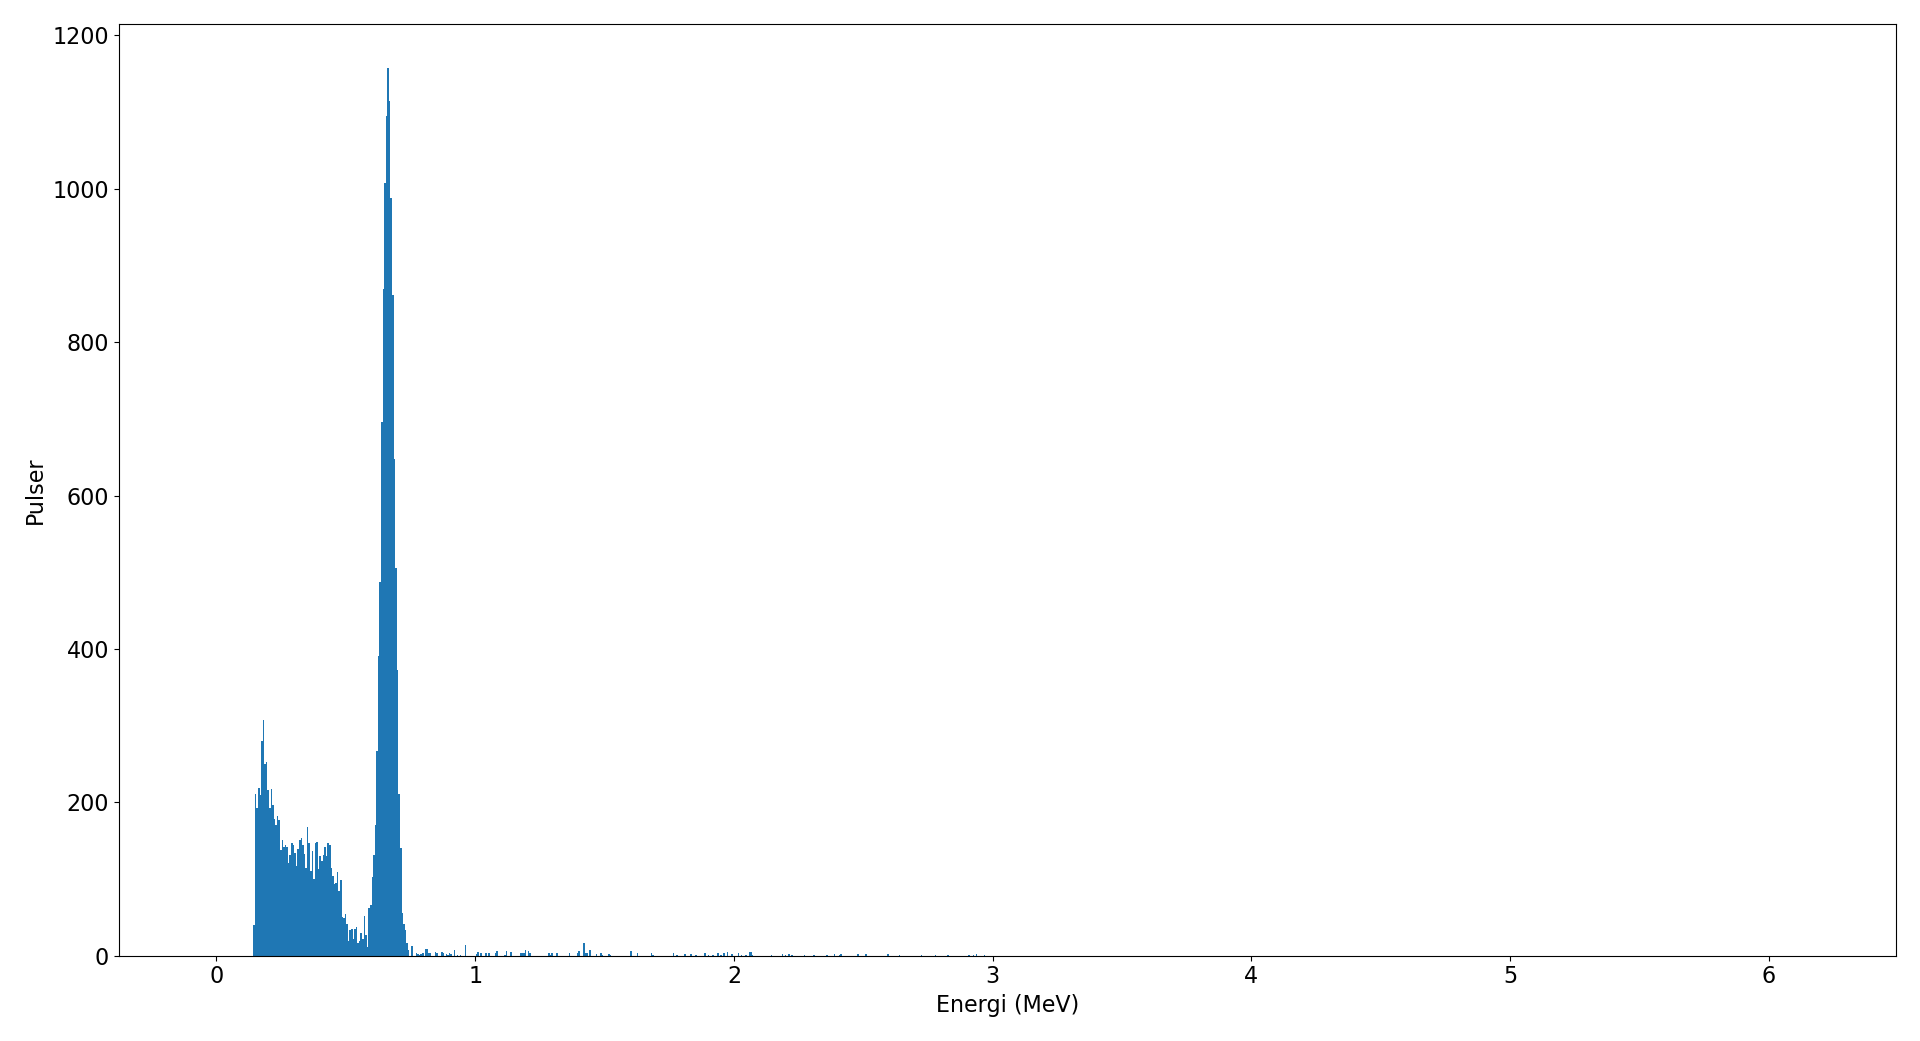
\includegraphics[width=\textwidth, keepaspectratio]{../images/mushrooms.png}
    \caption{Gammaspektrum, svamp från Kiev 2002.}
    \label{fig:mushrooms}
\end{figure}

\begin{figure}[!hp]
    \centering
    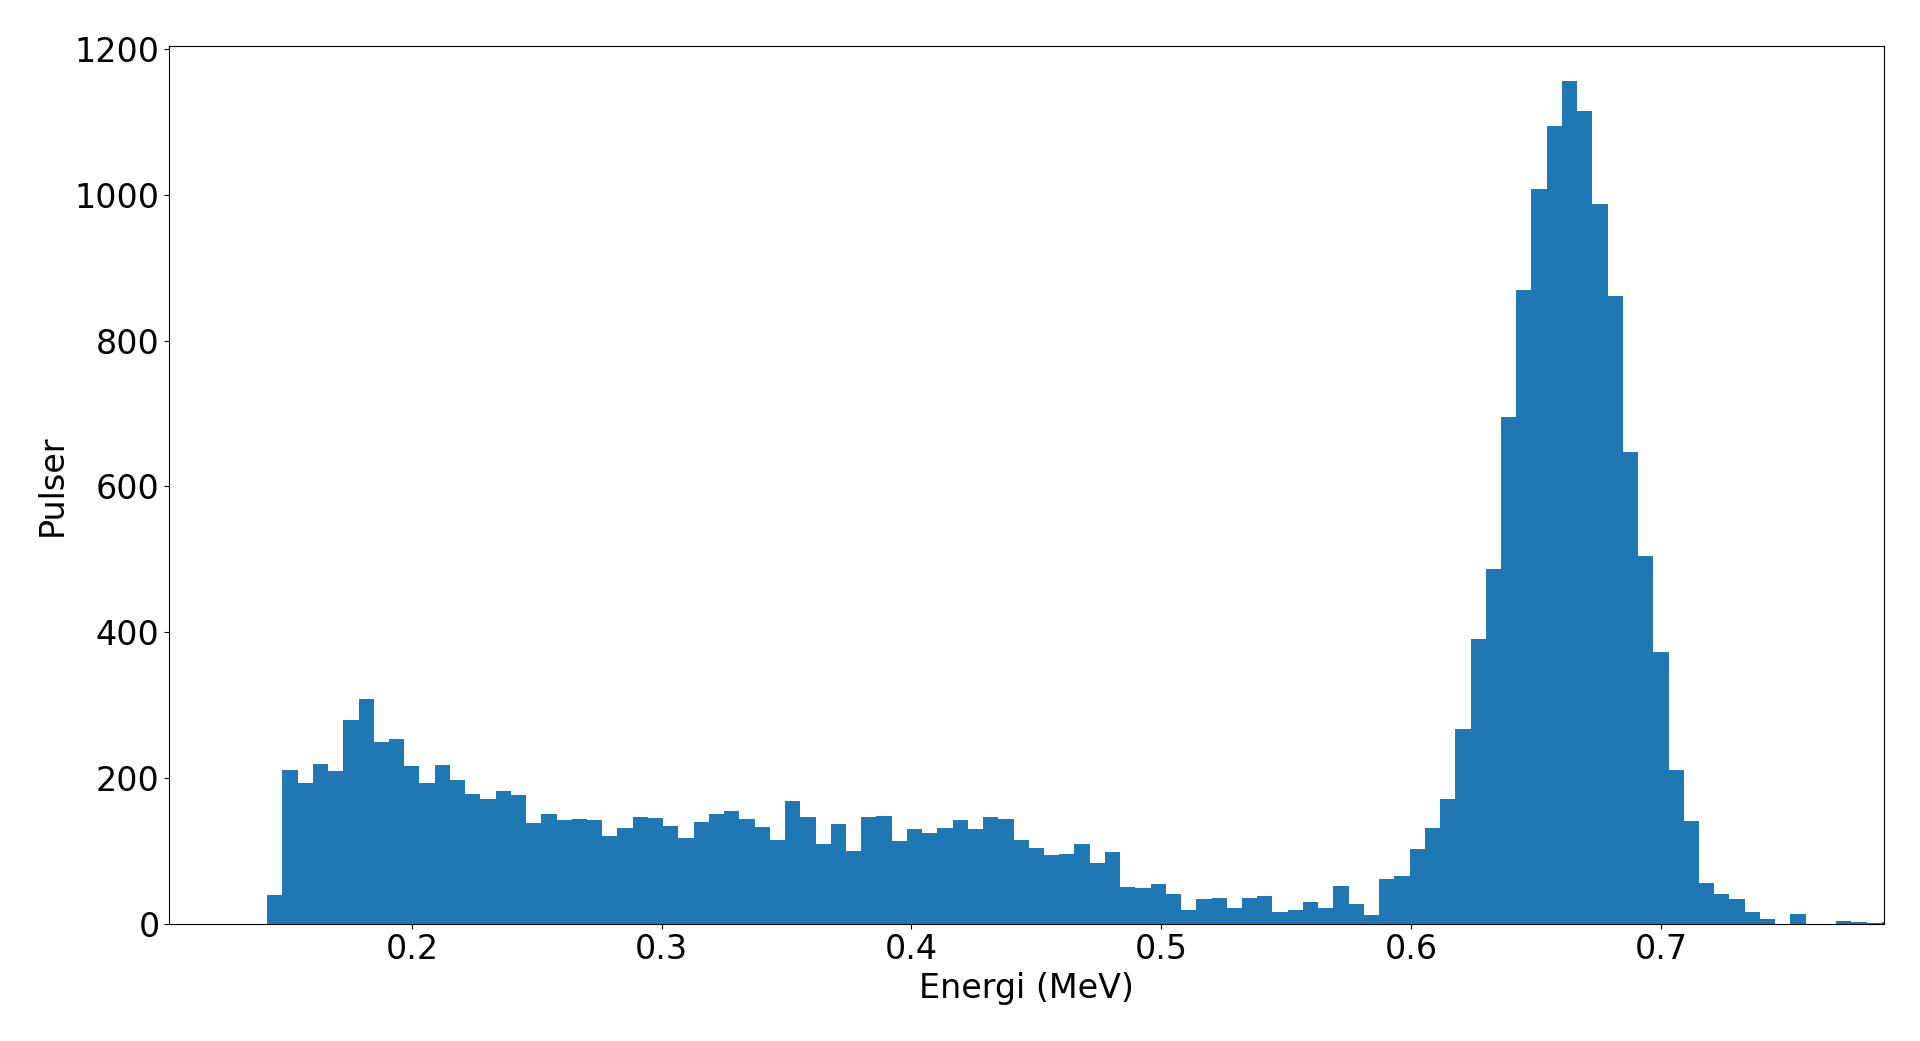
\includegraphics[width=\textwidth, keepaspectratio]{../images/mushrooms_zoom.png}
    \caption{
        Förstoring av största koncentration från figur~\ref{fig:mushrooms}.
        Intervallet visat är \qtyrange{0}{0.8}{\MeV}.
    }
    \label{fig:mushroomszoom}
\end{figure}

\begin{figure}[!hp]
    \centering
    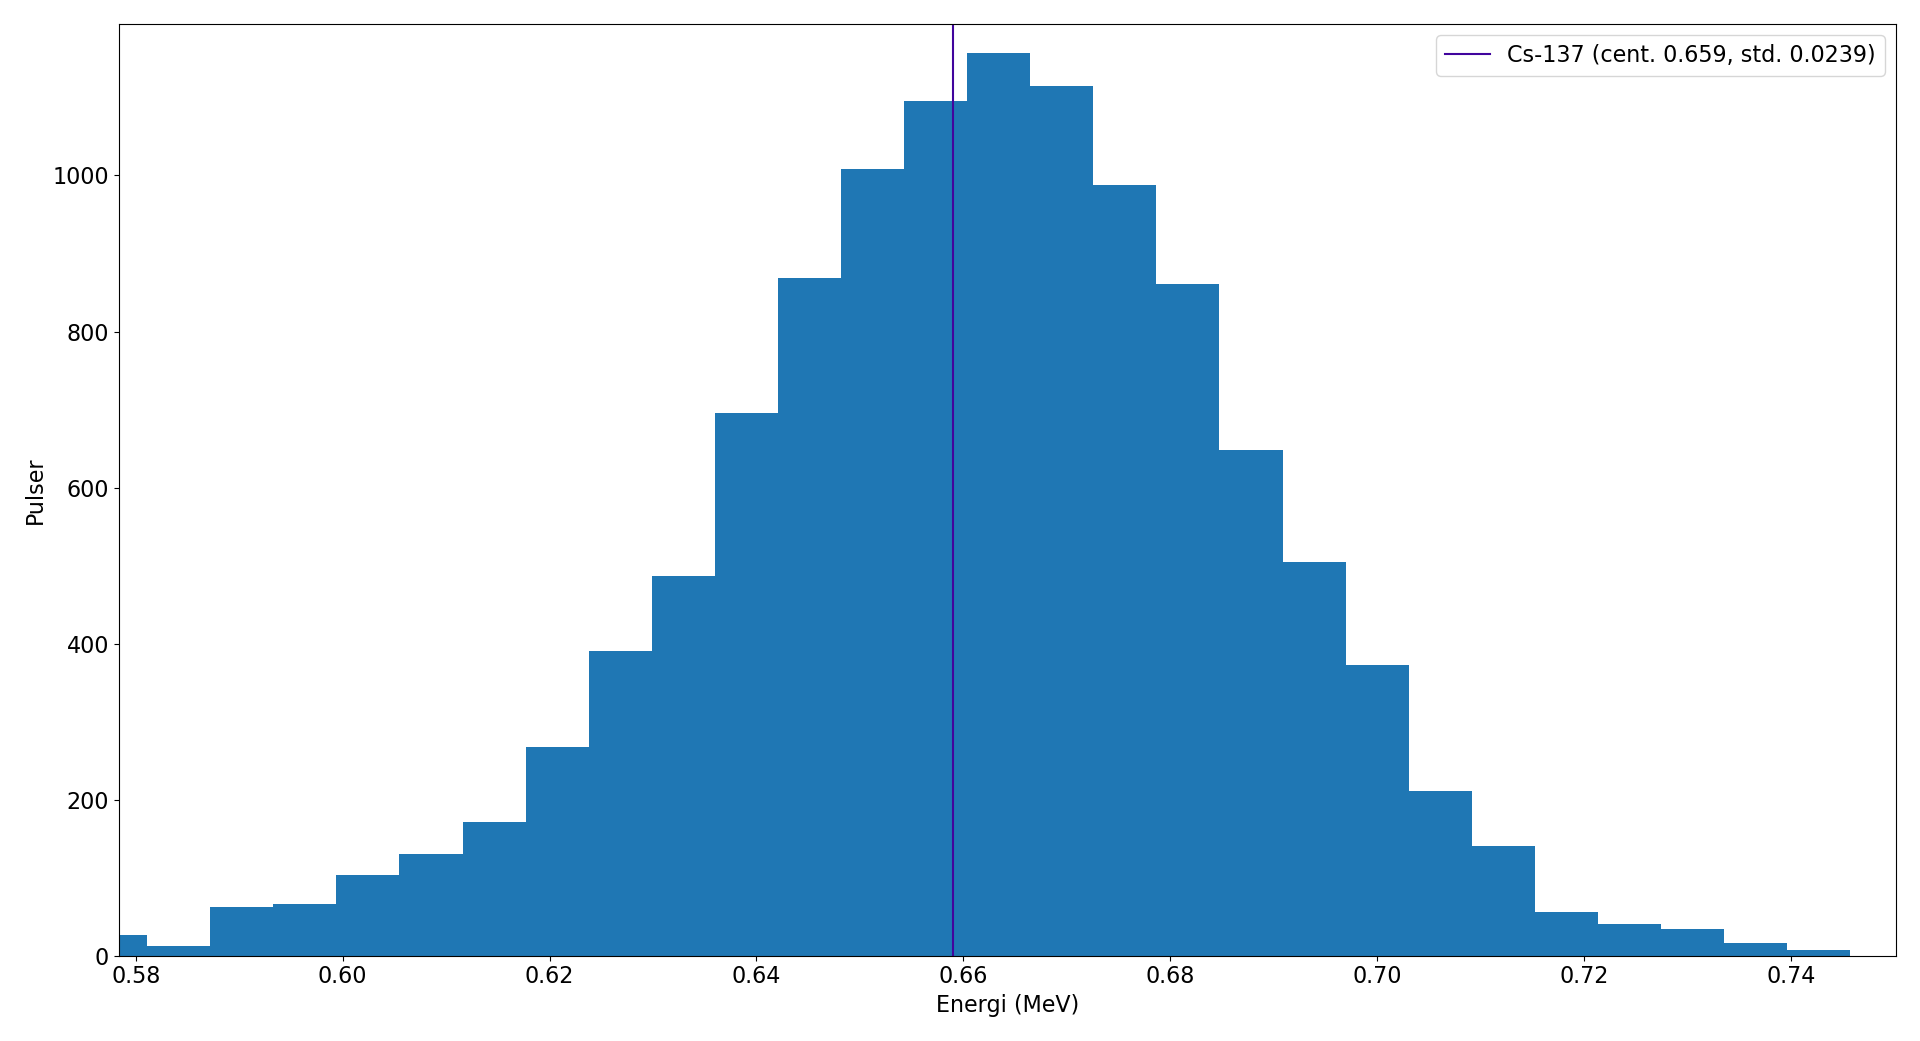
\includegraphics[width=\textwidth, keepaspectratio]{../images/mushrooms_top.png}
    \caption{
        Förstoring av topp från figur~\ref{fig:mushrooms}.
        Intervallet visat är \qtyrange{0.58}{0.75}{\MeV}.
    }
    \label{fig:mushroomstop}
\end{figure}

Toppens form tyder på en normalfördelning med centroid vid \qty{0.659}{\MeV},
standardavvikelse på \qty{0.0239}{\MeV} och FHWM på \qty{0.0544}{\MeV}. Dessa
värden föreslår att provet mycket riktigt innehåller Cs-137 vars sönderfall ger
upphov till fotoner med energinivåer på \qty{0.661657}{\MeV} (se
avsnitt~\ref{sec:theory}) (felmarginal \qty{0.40}{\percent}).

De större pulserna med lägre energi än toppen (se
figur~\ref{fig:mushroomszoom}) förklaras genom Comptonspridning, för vilken
vi noterar en bakåtspridningstopp vid \qty{0.8}{\MeV} och en Comptonkant kring
\qty{0.48}{\MeV}. Övriga pulser förklaras genom slumpartad bakgrundsstrålning
och är försumbara.

\subsubsection{Gammastrålning i salt} \label{sec:salt}

Figur~\ref{fig:salt} visar mätresultaten från saltprovet. Pulserna tycks vara
mestadels i intervallet \qtyrange{0.1}{1.6}{\MeV}. Figur~\ref{fig:saltzoom}
visar en förstoring av detta område. En topp syns nära \qty{1.45}{\MeV}.
Figur~\ref{fig:salttop} visar en förstoring av denna topp.

\begin{figure}[!hp]
    \centering
    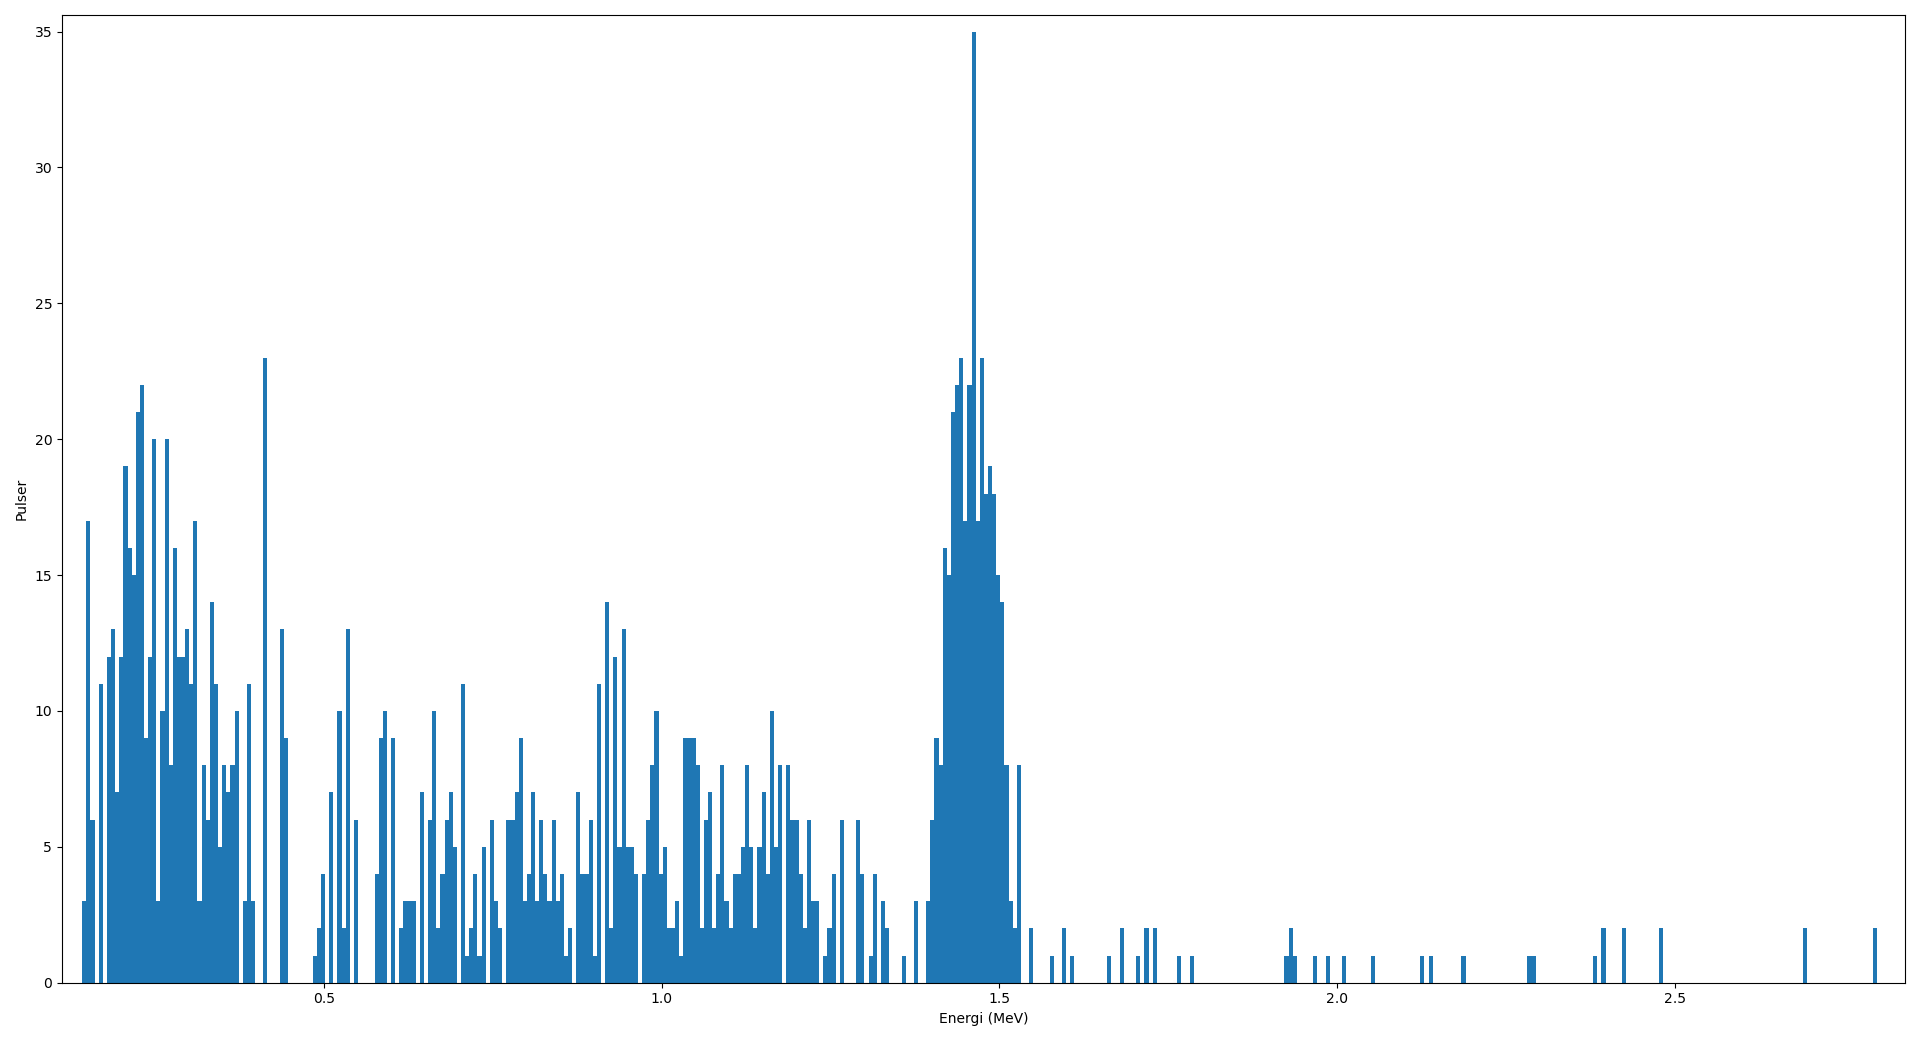
\includegraphics[width=\textwidth, keepaspectratio]{../images/salt.png}
    \caption{Gammaspektrum, mineralsaltet Seltin.}
    \label{fig:salt}
\end{figure}

\begin{figure}[!hp]
    \centering
    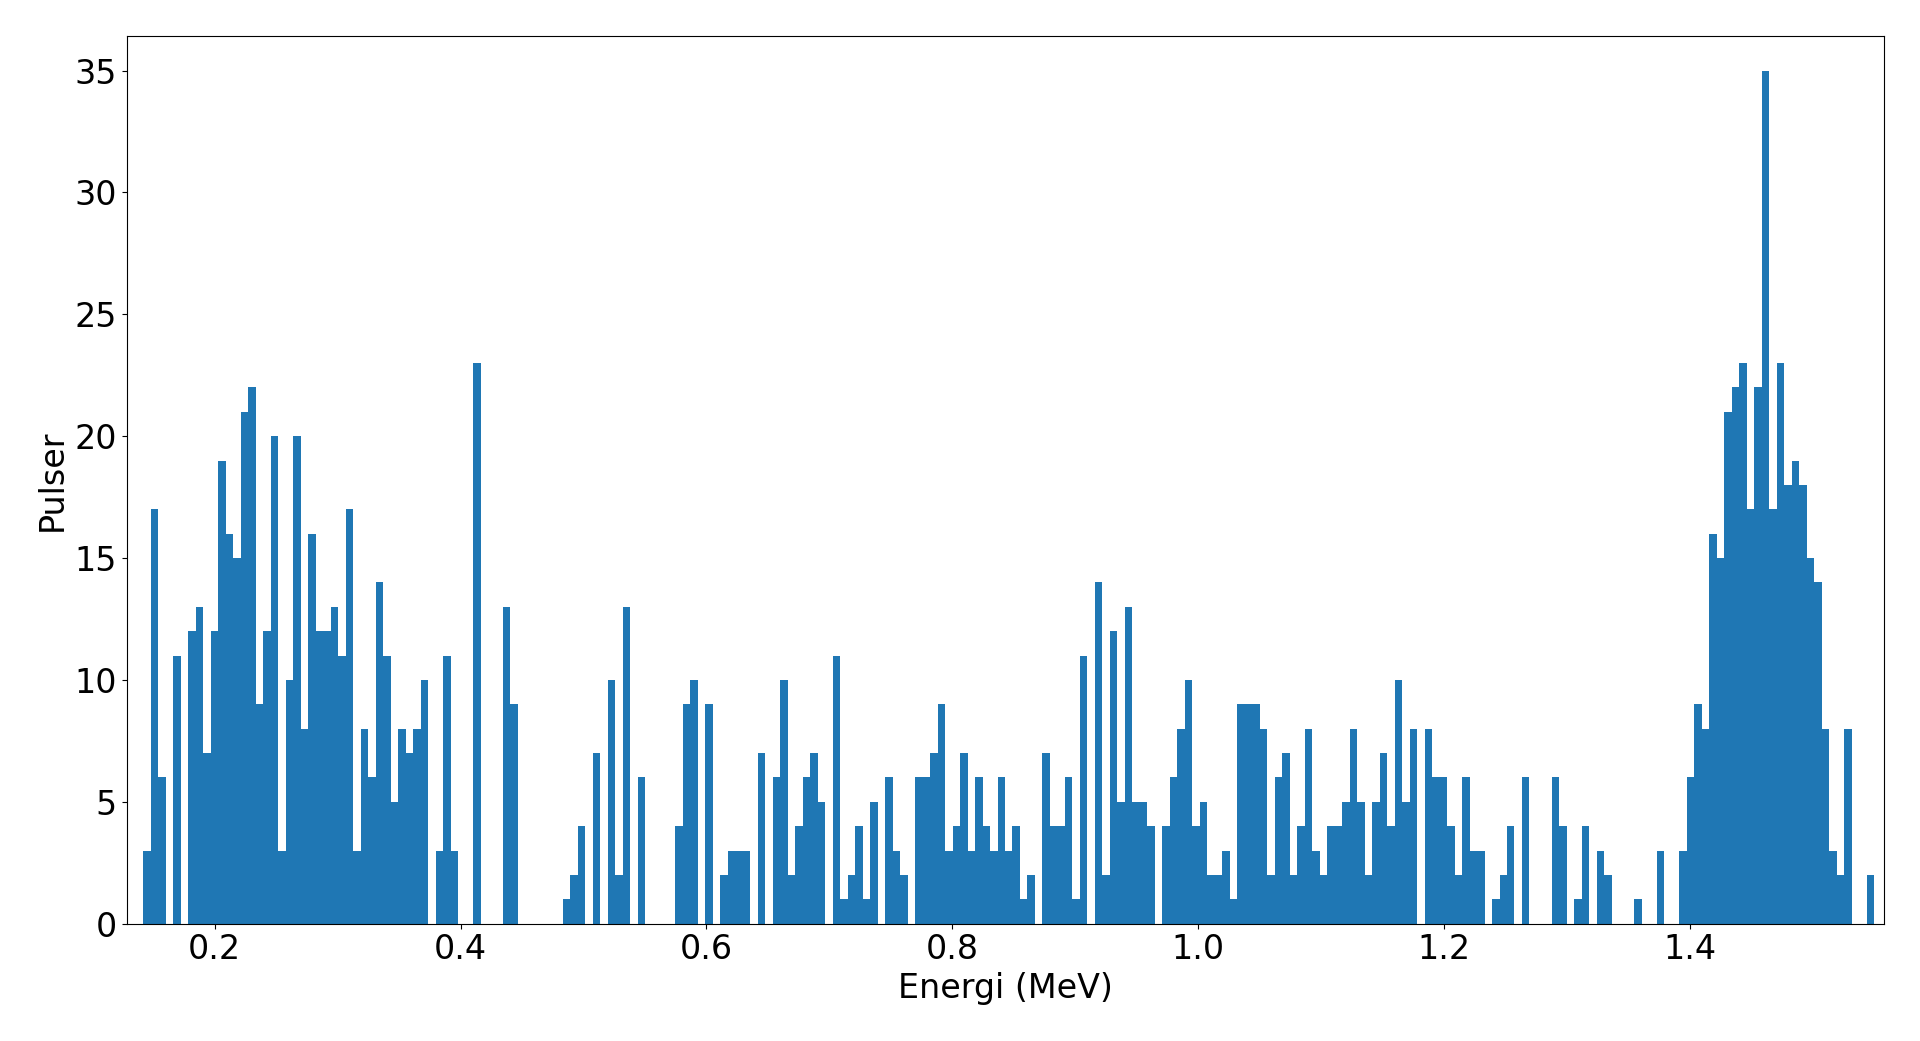
\includegraphics[width=\textwidth, keepaspectratio]{../images/salt_zoom.png}
    \caption{
        Förstoring av största koncentration från figur~\ref{fig:salt}.
        Intervallet visat är \qtyrange{0.1}{1.6}{\MeV}.
    }
    \label{fig:saltzoom}
\end{figure}

\begin{figure}[!hp]
    \centering
    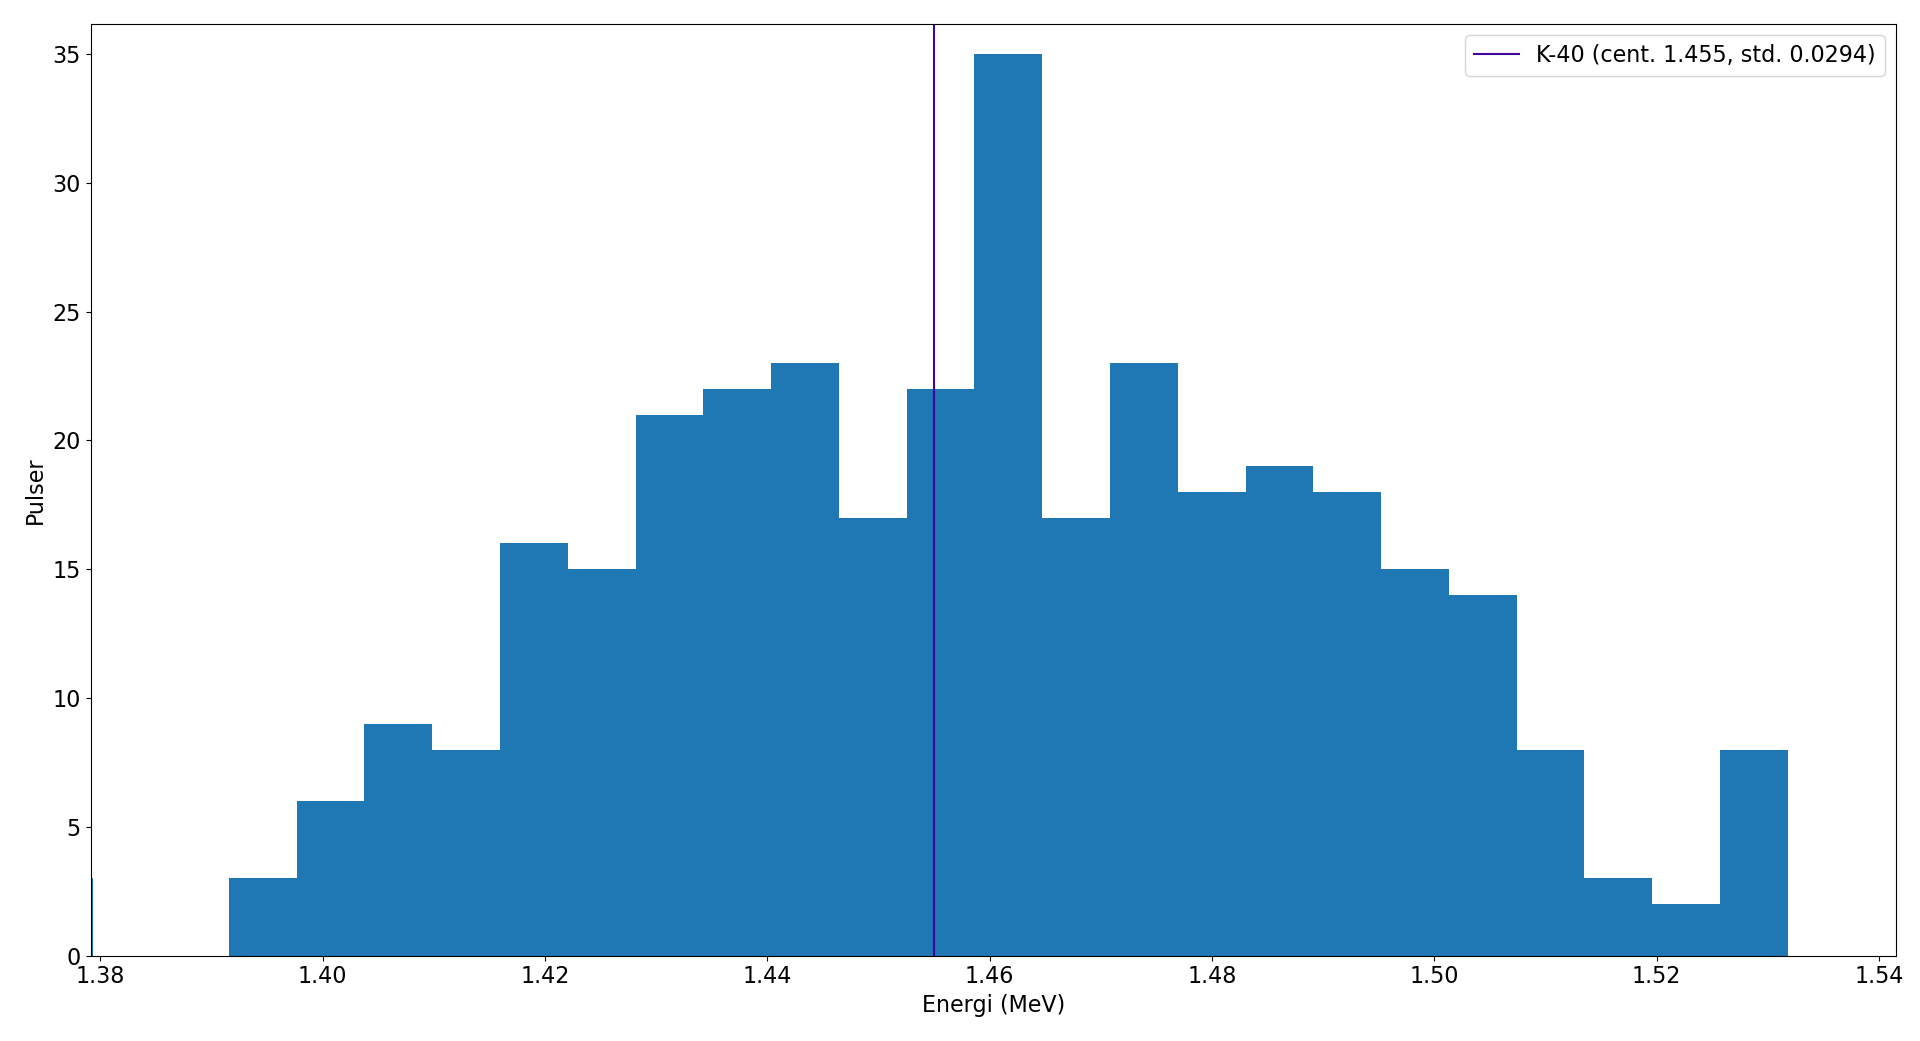
\includegraphics[width=\textwidth, keepaspectratio]{../images/salt_top.png}
    \caption{
        Förstoring av topp från figur~\ref{fig:salt}.
        Intervallet visat är \qtyrange{1.38}{1.54}{\MeV}.
    }
    \label{fig:salttop}
\end{figure}

Toppens form tyder även här på en normalfördelning med centroid vid
\qty{1.455}{\MeV}, standardavvikelse på \qty{0.0294}{\MeV} och FHWM på
\qty{0.0640}{\MeV}. Dessa värden föreslår att provet mycket riktigt innehåller
K-40 vars sönderfall ger upphov till fotoner med energinivåer på
\qty{1.460822}{\MeV} (se avsnitt~\ref{sec:theory}) (felmarginal
\qty{0.40}{\percent}).

Likt med svampens spektrum visas antydan till Comptoneffekten med en
bakåtspridningstopp nära \qty{0.25}{\MeV} och en Comptonkant kring
\qty{1.2}{\MeV}. Bakgrundsstrålningen antas ha försumbar påverkan.

Till skillnad från svampens spektrum har detta betydligt mer brus. Detta beror
främst på att färre pulser detekterades. Tabell~\ref{tab:samples} visar att
svampprovet gav av pulser med cirka \num{13} gånger högre frekvens, för ett
slutresultat på cirka \num{35} gånger fler pulser. För vidare analys se
avsnitt~\ref{sec:analysis}.

\subsubsection{Betastrålning i stav} \label{sec:cesium}

Figur~\ref{fig:cesium} visar mätresultaten från cesiumprovet. Pulserna är
mestadels i intervallet \qtyrange{0.1}{0.7}{\MeV}. Figur~\ref{fig:cesiumzoom}
visar en förstoring av detta område. Två toppar syns nära
\qtylist{0.62;0.65}{\MeV}. Figur~\ref{fig:cesiumtop} visar en förstoring av
dessa toppar.

\begin{figure}[!hp]
    \centering
    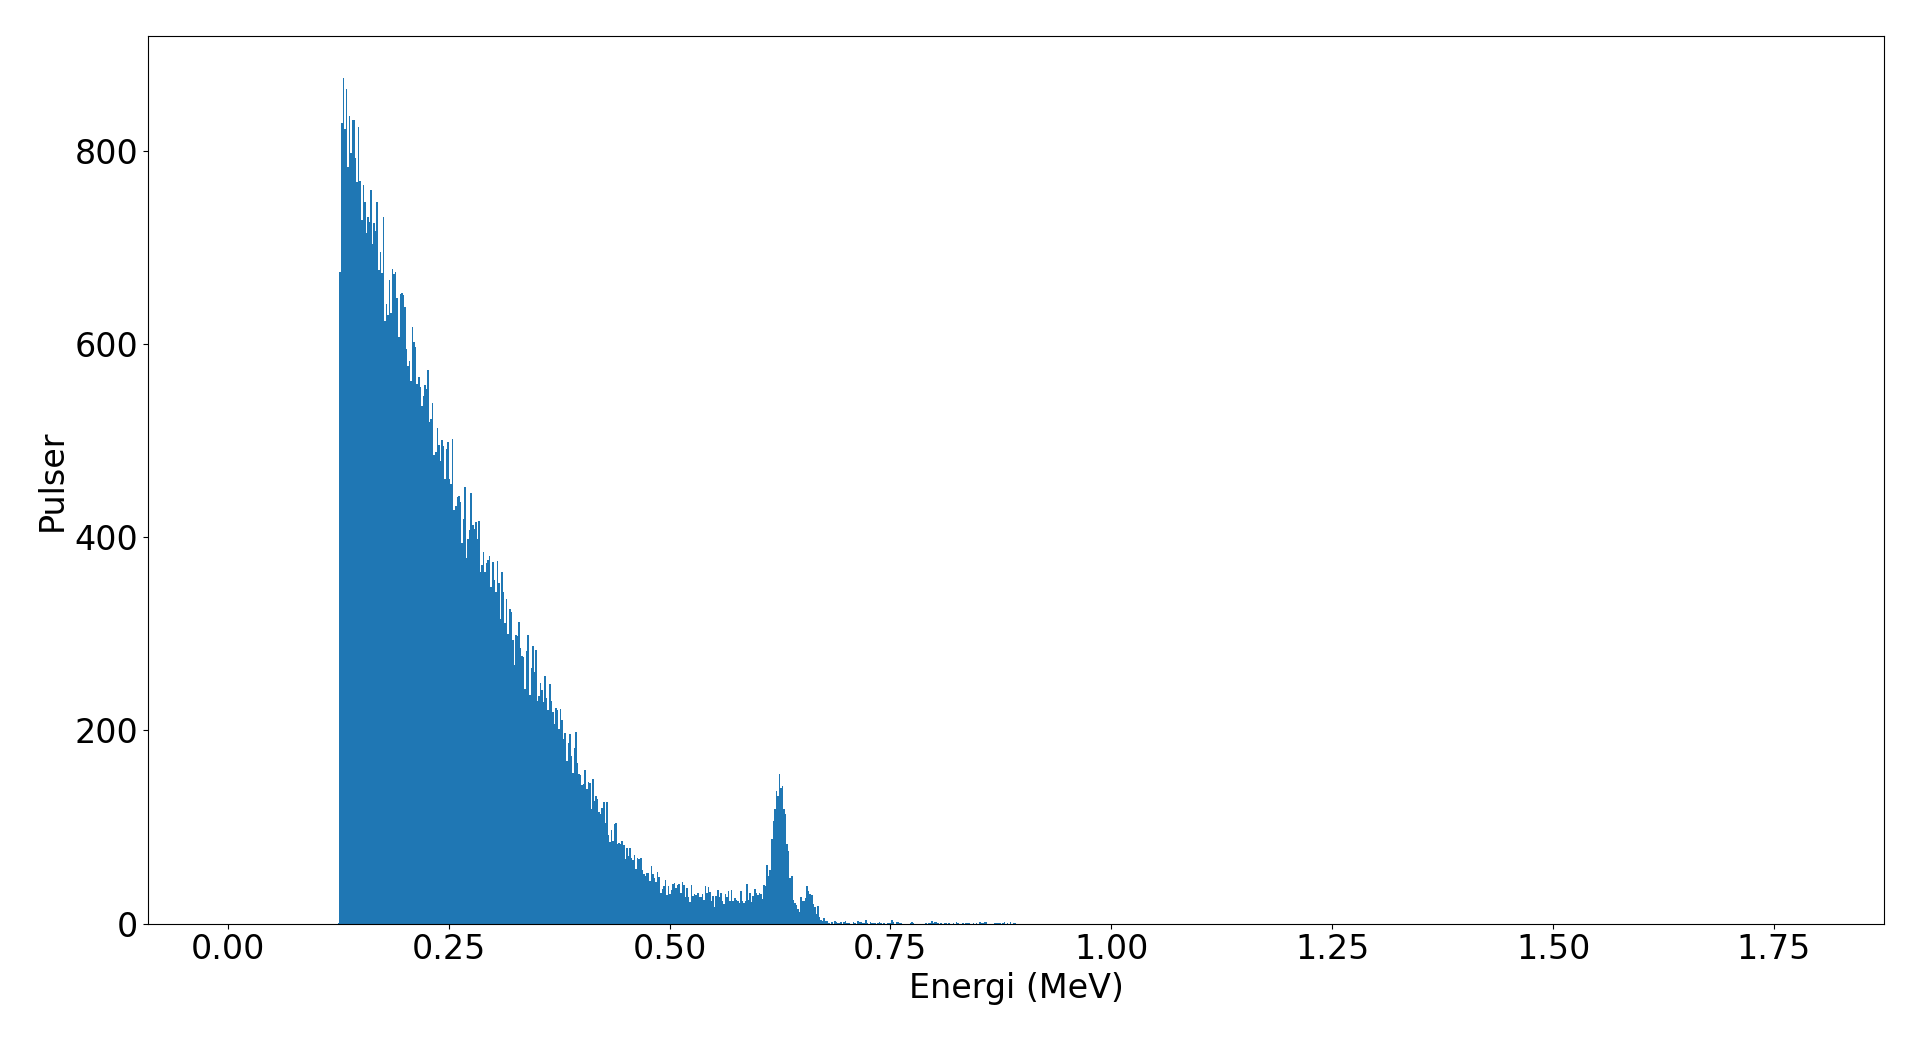
\includegraphics[width=\textwidth, keepaspectratio]{../images/cesium.png}
    \caption{Betaspektrum, Cs-137.}
    \label{fig:cesium}
\end{figure}

\begin{figure}[!hp]
    \centering
    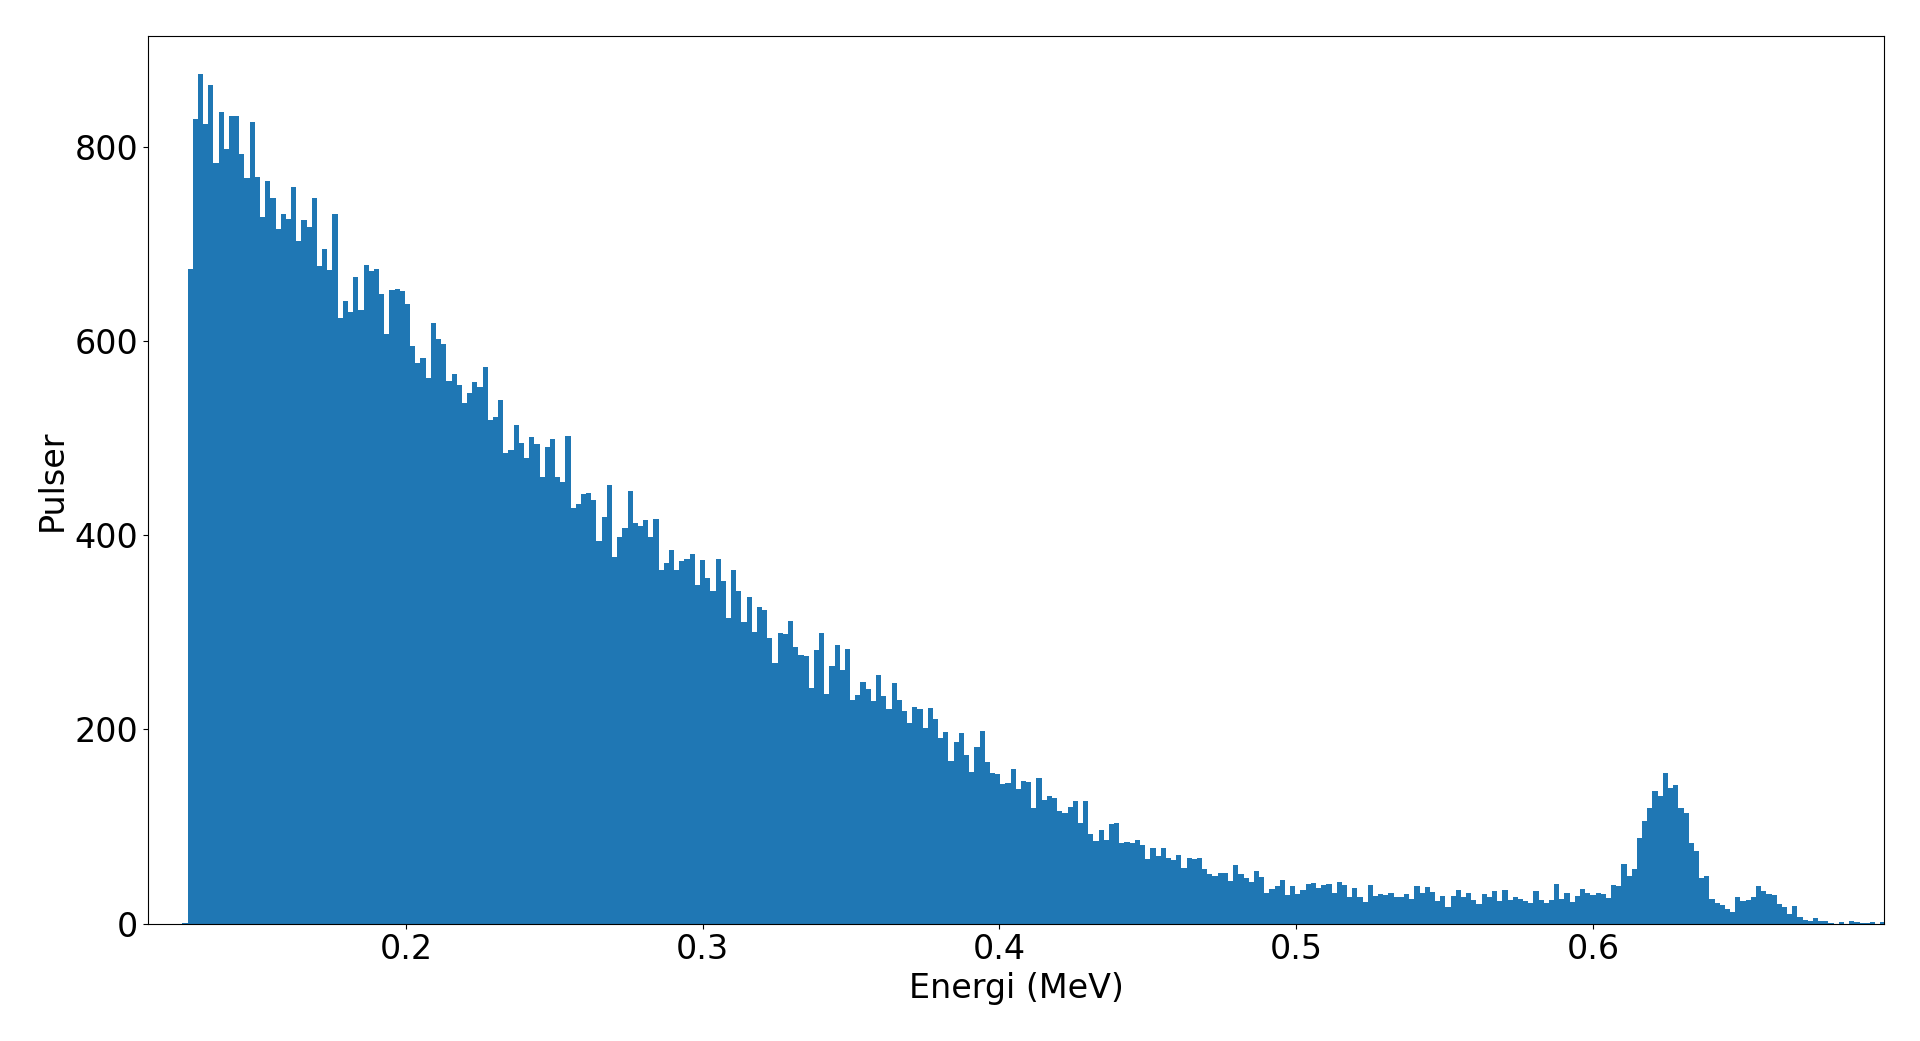
\includegraphics[width=\textwidth, keepaspectratio]{../images/cesium_zoom.png}
    \caption{
        Förstoring av största koncentration från figur~\ref{fig:cesium}.
        Intervallet visat är \qtyrange{0.1}{0.7}{\MeV}.
    }
    \label{fig:cesiumzoom}
\end{figure}

\begin{figure}[!hp]
    \centering
    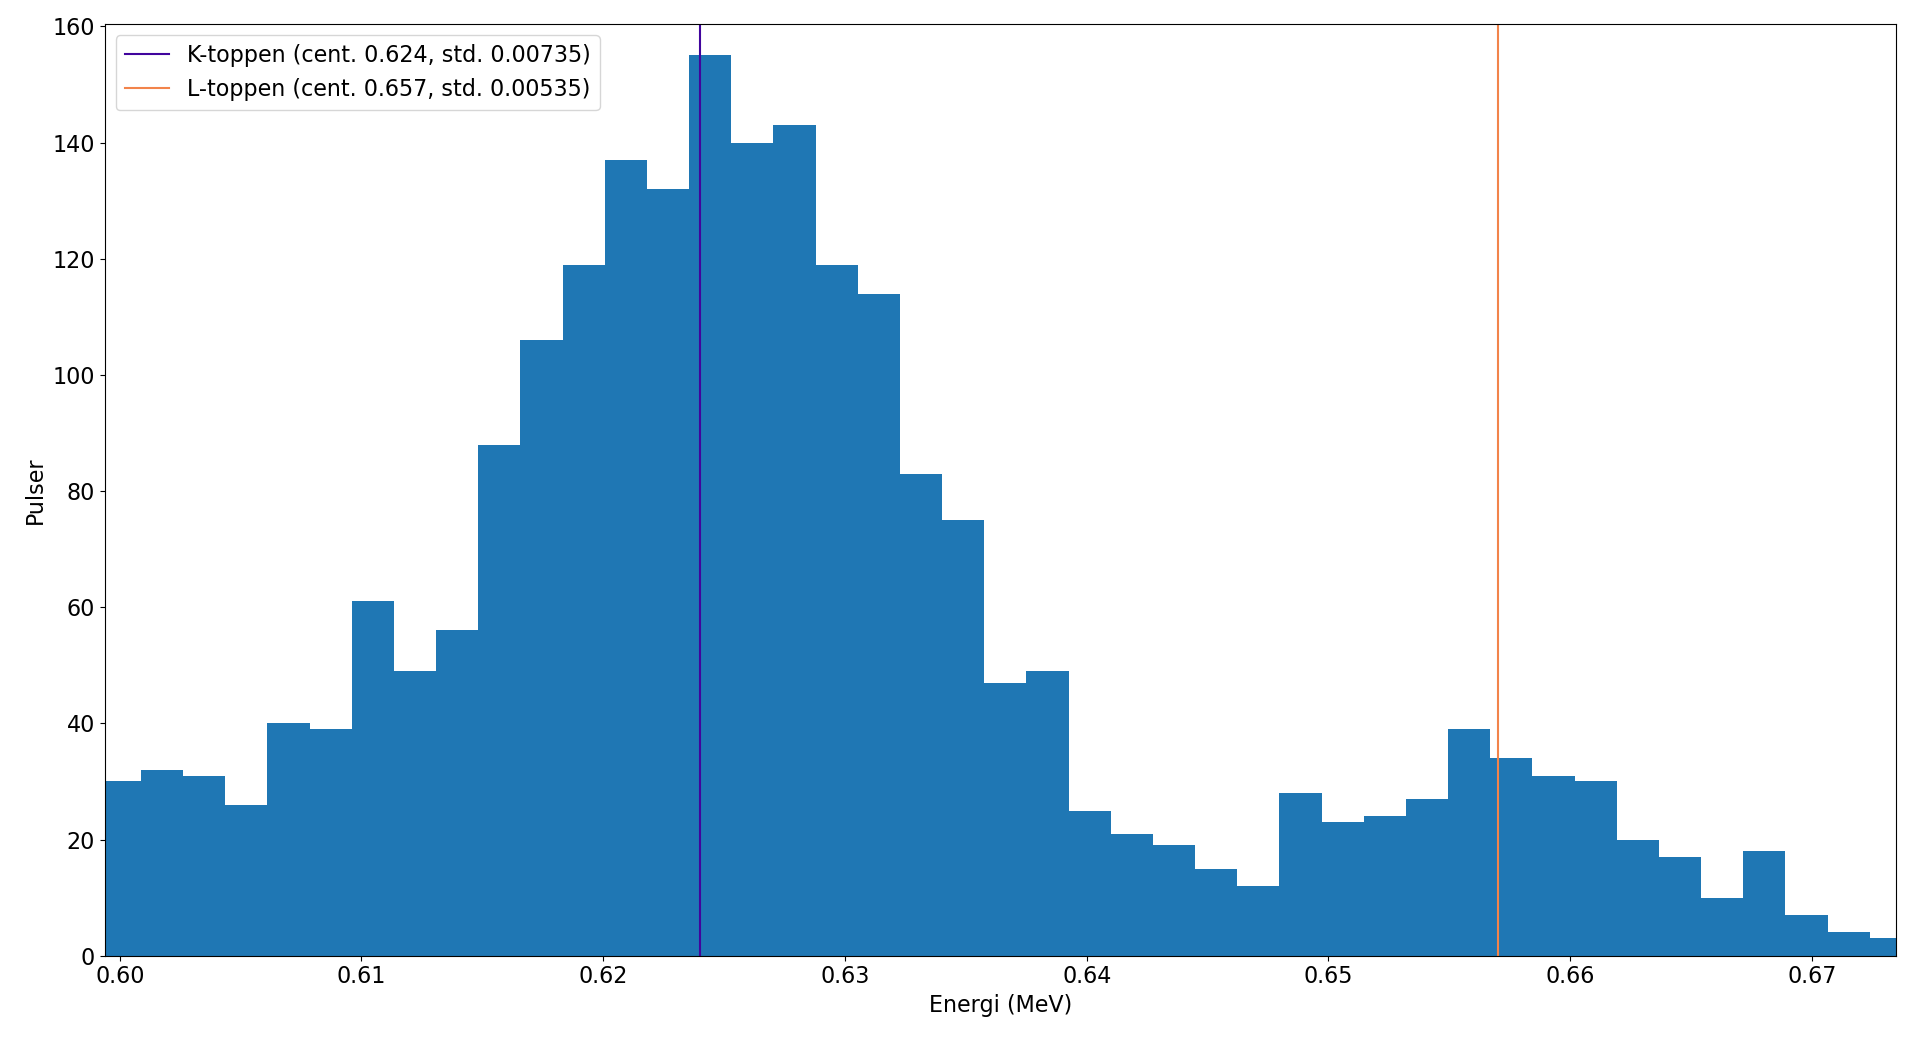
\includegraphics[width=\textwidth, keepaspectratio]{../images/cesium_top.png}
    \caption{
        Förstoring av toppar från figur~\ref{fig:cesium}.
        Intervallet visat är \qtyrange{0.605}{0.675}{\MeV}.
    }
    \label{fig:cesiumtop}
\end{figure}

Topparnas former tyder återigen på normalfördelningar med centroioder vid
\qtylist{0.624;0.657}{\MeV}, standardavvikelser på
\qtylist{7.35;5.35}{\kilo\eV} och FHWM på \qtylist{0.0172;0.0138}{\MeV}.
Dessa antas motsvara elektronerna som avges som följd av inre konversion från
K- respektive L-skalen och har kalibrerats utifrån detta (se
avsnitt~\ref{sec:theory}~och~\ref{sec:method}).
